\section{Theorie}
\label{sec:Theorie}
Der Untraschall wird vielfach in der zerstörungsfreien Werkstoffprüfung und in der Medizin angewendet.\\
\noindent Schall ist eine aufgrund von Druckschwankung fortbewegende longituale Welle

\begin{equation}
    p(x,t) = p_0 +v_0 Z cos(wt-kx)\\
\end{equation}
\noindent (die akustische Impedanz (Schallkennwiderstand) $Z=c\cdot p$, $p$ = Dichte des durchstrahlten Materials, $v$ =
die Schallgeschwindigkeit Impedanz Material).\\
\noindent
Schallwellen verhalten sich ähnlich wie elektromagnetische Wellen. Daher ist die Schallgeschwindigkeit aufgrund der Druck- bzw. Dichteänderungen materialabhängig.
Der Schall enspricht in Gasen und  Flüssigkeiten einer longitudinalen Welle und in Festkörpern aufgrund der Schubspannungen sowohl einer longitudialen als auch transversalen Welle.
Die Schallgeschwindigkeit wird folglich beschrieben mit:

\begin{equation}
    c_{\text{Fl}} = \sqrt{\frac{1}{\kappa \cdot \rho}}\\
\end{equation}
\noindent ($\kappa$ = Kompressibilität, $\rho$ = Dichte)  
\begin{equation}
    c_{\text{Fe}} = \sqrt{\frac{E}{ \rho}}\\
\end{equation} 

\noindent ($E$= Elastizitätsmodul).\\
\noindent 
Schallgeschwindigkeiten in Festkörpern sind richtungsabhängig.\\
\noindent
Bei der Schallausbreitung nimmt die Intensität der Schallwellen  aufgrund dem durch Absorption verlierenden Energieteil  exponentiell nach der Strecke $x$ Absorption ab
\begin{equation}
    I(x) = I_0 \cdot e^{- \alpha x }\\
\end{equation}
\noindent ($\alpha$ = Absorptionskoeffizient der Schallamplitude). \\
\noindent Bei Luft ist diese Abschwächung sehr stark, weswegen ein Kontaktmittel verwendet wird.\\
\noindent Die Eigenschaft der Reflexion von Wellen gilt auch beim Schall (Reflexion auf eine Grenzfläche zwischen 2 Materialien).
 Der Reflexionskoeffizient $R$ ergibt sich dabei nach
\begin{equation}
    R= {\Bigl(\frac{Z_1-Z_2}{Z_1+Z_2}\Bigr)}^2.\\
\end{equation}
\noindent
Der transmittierte Anteil $T$ ist dann $T= 1-R$.\\
\noindent 
Die Anwendung des reziproken piezo-elektischen Effektes ist eine mögliche Methode bei Erzeugung des Untraschalls. Die piezoelektrischen Kristalle können, wenn sie in
ein elektrisches Wechselfeld gebracht werden und eine ihrer polaren Achsen in Richtung des elektrischen Feldes zeigt, zu Schwingungen angeregt werden, wobei der Ultraschall entsteht. Wenn die Anregungsfrequenz mit der Eigenfrequenz übereinstimmt, kommt es zur
Resonanz, und es werden sehr große Schwingungsamplituden erreicht. Als Empfänger des Ultraschalls kann ebenfalls wieder ein piezoelektrischer Kristall genutzt werden, der durch Auffangen des Ultraschalls in Schwingung versetzt wird.\\
\noindent In der Ultraschalltechnik werden zwei Verfahren mit Laufzeitmessungs-Prinzip angewendet (das Durchschallungs- und das Impuls-Echo-Verfahren), um mit dem Ultraschall Informationen über ein zu
untersuchendes Objekt zu bekommen.\\
Beim Durchschaltungs-Verfahren ist der Ultraschallsender an einem Ende des Probenstücks und der Ultraschallempfänger am anderen Ende. Es wird ein kurzzeitiger Schallimpuls ausgesendet. 
Am Ultraschallempfänger wird eine aufgund einer Fehlstelle in der Probe abgeschwächte Intensität gemessen. Eine genaue Ortsbestimmung dieser Fehlstelle ist nicht möglich.\\
\begin{figure}[H]
    \begin{center}
    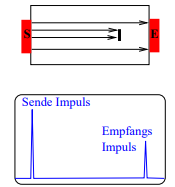
\includegraphics[width = 4cm, height= 4cm]{Durchschaltungsverfahren.png}
    \caption{Durchschaltungs-Verfahren.\protect\cite{AL}}
    \end{center}
    \label{fig:Durchschaltungsverfahren}
    \end{figure}
    \noindent
Beim Impuls-Echo-Verfahren befindet sich der Ultraschallsender auch als Ultraschallempfänger an einem Ende des Probenstücks. An einer Grenzfläche wird der Schallimpuls reflektiert und dann vom Empfänger
aufgenommen.  Die Höhe des Echos wird Aufschlu"s  über die Grö"se der Fehlstelle gegeben. Die Lage der Fehler wird über
 
\begin{equation}
    s= \frac{1}{2} ct\\
\end{equation}
\noindent bestimmt.
\begin{figure}[H]
    \begin{center}
    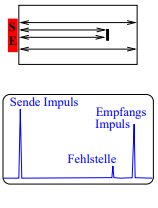
\includegraphics[width = 4cm, height= 4cm]{Impulsecho.png}
    \caption{Impuls-Echo-Verfahren.\protect\cite{AL}}
    \end{center}
    \label{fig:Impulsecho}
    \end{figure}
    \noindent
Die Laufzeitdiagramme können in einem A-Scan, B-Scan oder einem  TM- Scan dargestellt werden.





